\chapter{基于用户画像的推荐系统综述}
	\section{引言}
	自从1992年著名的施乐公司的科学家们为了解决困扰已久的信息负载问题,第一次从概念上提出协同过滤的算法模型。1998年,林登及其同事们成功申请了item协同过滤技术的专利,经过多年的工程实践,美国电商亚马逊公司的工程师们骄傲的宣称:在公司所有的销售量,推荐系统占比已经占到整个Gross Merchandise Volume的百分之三十以上。不久之后的美国公司Netflix,因为其创始人与前任公司签署有若干年内不得从事同行工作的限制,于是通过举办推荐算法优化竞赛绕开限制,用以开发出更好的推荐算法。此次竞赛吸引了数以千计的团队参与角逐,期间进行了上百种的算法模型组合、优化的尝试,虽然Netflix公司为冠军团队支付了百万美金,回报是Netflix推荐系统的快速发展以及营收的俩位数增长。其中冠军团队凭借Sigular Value Decomposition和Gavin Potter跨界的引入心理学的方法进行的组合算法模型,在诸多优秀团队中脱颖而出。其中,矩阵分解的核心是将一个非常稀疏的用户评分矩阵R分解为两个更小的矩阵:只包含User特性的矩阵P和只包含Item特性的矩阵Q,利用P和Q相乘的结果R'来拟合原来的评分矩阵R,使得矩阵R'在R相同位置之间的损失函数值尽量的小,通过定义一个R和R'之间的距离定义(一般为曼哈顿距离),如果矩阵R'是正定矩阵,那么把矩阵分解转化成梯度下降求解的局部最优解,就是全局最优解。与此同时,Pandora、LinkedIn、Hulu等网站在个性化推荐领域都展开你争我抢的竞争势头,使得推荐系统在各个细分行业、垂直领域开始全面开花,都有了不少爆发性进展。但是,对于拥有全品类的综合性购物电商、广告营销,推荐系统的进展还是缓慢,主要原因是因为不同类型的商品,消费者的心态也是不同的,例如大型家电,消费者肯定是先看了又看、选了又选,从价格、定位、功能到噪声比、性价比,大多数都会先做足了调查,才会购买;与此相反,对于日常用品消费者可能眼睛都不眨就购买了,对于这俩种极端的消费情况,推荐系统需要做出截然不同的推荐策略,具体的,单个模型在母婴品类的推荐效果还比较好,但在其他品类就可能很差,很多时候需要根据场景、推荐栏位、品类等不同,设计不同的推荐模型。同时由于用户兴趣随时间会不停的变动,需要一种机制,使得推荐系统能定期对数据进行评估、分析,要命的是对于不同类型的商品有不同的更新频率,这就对推荐系统提出了更加智能化的挑战。还有,如果定期更新模型,则可能会因为计算资源的限制导致无损害推荐的实时性,因为模型训练也要相当cpu计算时间,而传统的Hadoop的方法实在是无法进行大的更新频率,spark框架又因为昂贵的内存限制了其计算容量,最终业务会到达一个数据量,此时的推荐效果会因为实时性问题达到第一个计算瓶颈。推荐算法包括基于人口统计学的推荐\citep{social-filter}、基于商品内容的推荐\citep{content-based}、基于user/item的协同过滤\citep{collab-filter}的推荐等。基于内容的推荐\citep{recmd_content_based}对物品冷启动问题免疫,但是无法解决用户冷启动问题\citep{cold-start},还有过拟合的问题:即在训练集上有比较好的表现,但在实际应用中效果往往不尽人意,推荐系统的通用性和移植性往往比较差,适合针对细分行业下的商品做推荐,一旦换了产品类型,往往需要构建新的模型。基于邻域的协同过滤算法,虽然没有领域知识要求,算法通用性好,但存在有冷启动问题、数据稀疏性问题。

	由此,笔者在实际工程中,针对传统推荐算法的种种弊端,选择了用户画像。伟大的数学家、计算机学家Knuth先生说:如果遇到一个不好搞定的问题,那么就该添加一层中间层,用以屏蔽掉问题。实际上,用户画像作为底层数据仓库和上层推荐系统的缓冲层,起的就是这种作用。

	\section{用户画像的研究现状}
		\subsection{用户画像的组成部分}
		基于内容和用户画像的个性化推荐,有两个实体:内容和用户。需要有一种文本机制联系这两者的东西,我们定义其为标签。内容特征文本化为标签即为内容特征化,用户兴趣文本化标签则称为用户特征化\citep{user-profile,user-profile1,user-profile2,user-profile3,user-profile4}。因此,对于基于用户画像的推荐,主要分为以下几个关键部分:
		\begin{enumerate}[(1)]
		\item 标签库

		标签是联系用户与物品、内容以及物品、内容之间的纽带,也是反应用户兴趣的重要数据源。标签库的最终用途在于对用户进行行为、属性标记。是将其他实体转换为计算机可以理解的语言关键的一步。标签库则是对标签进行聚合的系统,包括对标签的管理、更新等。在用户画像的过程中有一个很重要的概念叫做颗粒度,就是我们的用户画像应该细化到哪种程度。举一个极端的例子,如果“用户画像”最细的颗粒度应该是细到每一个用户每一具体的生活场景中,但是这基本上是一个不可能完成的任务,同时如果用户画像的颗粒度太大,对于产品设计的指导意义又相对变小了,所以把握好画像的总体丰富程度显得异常重要了。可通过调查问卷的形式来减小颗粒度。一般来说,标签是以层级的形式组织的。如体育为一级维度、篮球为二级维度、NBA篮球为三级维度等。

		\item 内容特征化

		内容特征化即给内容打标签。目前有两种方式:人工打标签和机器自动打标签。针对机器自动打标签,需要采取机器学习的相关算法来实现,即针对一系列给定的标签,给内容选取其中匹配度最高的几个标签。这不同于通常的分类和聚类算法\citep{recmd-kmeans}。可以采取使用分词 + Word2Vec来实现,过程:将文本语料进行分词,以空格,tab隔开都可以,使用结巴分词。使用word2vec训练词的相似度模型。使用tfidf提取内容的关键词A,B,C。遍历每一个标签,计算关键词与此标签的相似度之和。取出TopN相似度最高的标签即为此内容的标签。

		\item 用户特征化

		用户特征化即为用户打文本标签。通过用户的行为日志和一定的模型算法得到用户的每个标签的权重。用户对内容的行为:点赞、不感兴趣、点击、浏览。对用户的反馈行为如点赞赋予权值1,默认为0,不感兴趣为-1;对于用户的浏览行为,则可使用点击、浏览作为权值。对商品发生的行为可以认为对此商品所有标签的行为。用户的兴趣是时间衰减的,即离当前时间越远的兴趣比重越低。时间衰减函数使用1/[log(t)+1], t为事件发生的时间距离当前时间的大小。要考虑到热门内容会干预用户的标签,需要对热门内容进行降权。
		\end{enumerate}

		\subsection{用户画像的构建周期}
		用户画像,即用户信息标签化,就是企业通过收集与分析消费者社会属性、生活习惯、消费行为等主要信息的数据之后,完美地抽象出一个用户的商业全貌作是企业应用大数据技术的基本方式。构建周期如\autoref{pic:userprofile_process}。
		\begin{figure}
	    \centering
	      \framebox{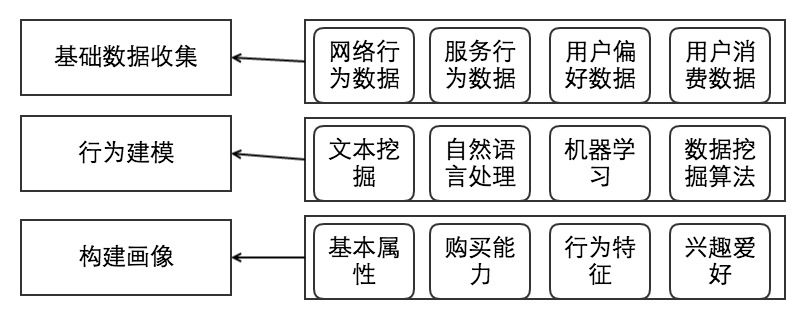
\includegraphics[scale=0.45]{figures/userprofile_process}}
	      \figcaption{用户画像的构建周期示意图}
	      \label{pic:userprofile_process}
	    \end{figure}
	    \begin{enumerate}[(1)]
	    \item 数据收集

	    数据收集大致分为四类:1、网络行为数据包括页面浏览量、活跃人数、访问时长、浏览注册转化率、注册活跃转换率等。服务内行为数据:点击浏览路径、网页停留时长、滑屏次数、滑屏频率、滑屏时长。用户内容偏好数据:点击、浏览、收藏内容、评价、评分、评论内容、社交内容、品牌偏好等。用户交易数据(交易类服务):购买率、折扣率、导流率、流失率等。收集到的数据没必要是百分之百的准确,大体差不多即可。应用中,具体就是在数据清洗阶段过滤一部分不靠谱的异常值,验证、更新数据这块需要在后面的阶段中建模来再判断,比如某用户在性别一栏填的女,但其语言数据显示其为男的概率更大,根据业务再选择丢弃数据还是更新数据。
	    
	    \item 行为建模

	    该阶段是对收集到数据进行建模,目标是抽象出用户的文本标签,这个阶段不应该再纠结数据的正确性,而是应该注重大概率事件,通过统计学假设检验尽可能地排除用户的偶然行为。这时也要用到数据挖掘算法模型,对用户的行为进行回归预测,比如已有一个线性回归函数:y=kx+b,X 代表用户行为,y是函数拟合的用户喜好度,y'是用户真实偏好,我们通过不断的训练数据,利用参数k和参数b来得出最新损失函数下的值,用以精确模拟y'。

	    \item 用户画像基本成型

	    该阶段是行为建模的深化,需要利用用户的基本属性,如性别、地域、年龄,得出用户更高层的抽象概念:消费能力、忠诚度、活跃度、社交爱好等。因为用户画像永远也无法百分百地拟合现实中的一个人,只能做的就是不断地去减小拟合的损失函数,因此,用户画像需要根据变化的基础数据不断修正已有的更高层的抽象概念,尽可能模拟用户的变化趋势。

	    \item 数据可视化

	    最后是数据可视化分析,这部分是最能体现推荐系统的产出,因为这是把用户画像真正的用视觉展示起来的一步,人类对数据不如对图画来的敏感,在此步骤中一般是针对群体做进一步的抽象,按照消费习惯、消费能力、消费偏好把用户归类为一类人,比如可以根据用户对价格的敏感度细分出高价值用户、核心用户、高忠诚用户。而决策层所做出的评估也应该是基于某一群体的潜在价值分布。典型的用户画像如\autoref{pic:user_profile}
	    \end{enumerate}
		\begin{figure}
	    \centering
	      \framebox{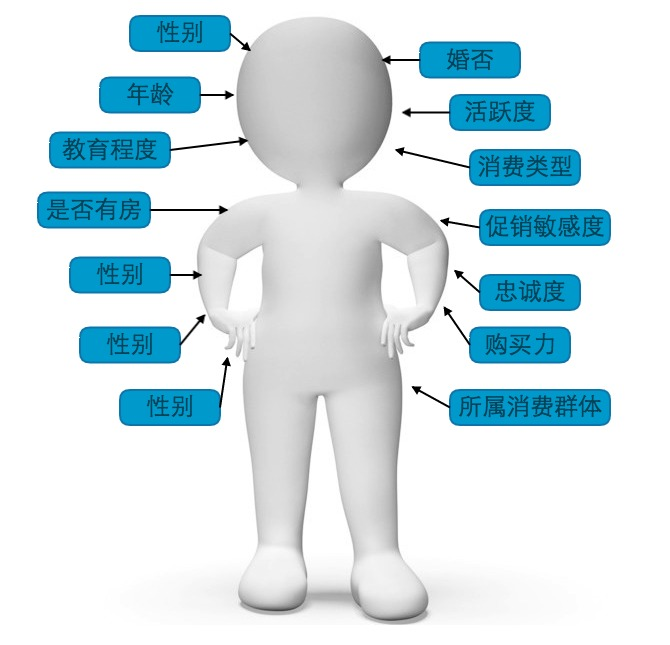
\includegraphics[scale=0.4]{figures/user_profile}}
	      \figcaption{用户画像示意图}
	      \label{pic:user_profile}
	    \end{figure}

		\subsection{用户画像的建模}
		用户画像的建模包括内容标签化和标签权重量化。建模过程:1、内容分析,从原先的物品描述信息中提取有用的信息用一种规范化的标签表示,有时候这种信息源自于作者提供的描述,有时候源自于用户的评价,不管如何,都需要人工审核验证正确性;2、上传、记录用户注册信息,生成用户基本信息,这些信息基本是不会变化的;上传、记录用户行为数据,这些数据是不断变化着的,通常是采用数据挖掘算法从潜在物品集合中取出若干个结果表示用户喜好的模型。例如,一个网页推荐系统,可以通过分析用户过往浏览过的文章,得出用户喜欢浏览类似于范冰冰的花边新闻,如果用户点击了所推荐的文章,则说明分析正确,否则需要根据反馈重新训练模型,从而实现一个反馈-推荐-反馈的闭环;3、推荐系统得出推荐集合后往往需要取topN,因为推荐系统的本质在精不在多。通过定义一个距离算法,匹配用户标签和商品标签的相关度,相关度一般正则为0-1之间,结果是一个二元的离散量:<pid,score>。根据相关度将生成一个用户潜在感兴趣的物品评分列表,然后去掉用户之前看过的商品,取topN即可。例如在电影用户画像的建模中,首先分析用户打分比较高的电影的共同特性,包括导演、演员、风格等,这些电影的标签就会成为此用户画像的一部分,根据打分的多少,给定一个合适的权重值。用户-标签用矩阵A表示,电影-标签用矩阵B表示,A乘B得出矩阵A,A中的一个元素即代表了一个用户与一部电影之间的相关度,固定一个用户,对所有相关度不为零的电影做排序,取topN即是推荐结果。用户画像建模的根本在于用户标签的获取和权重的定量分析。

		对于商品描述,也可以做进一步的处理,丰富商品的标签集合。其实和文本处理类似,笔者选择使用目前应用最广泛的方法:TF-IDF方法。设有N个文本文件,关键词$k_{i}$在$n_{i}$个文件中出现,设$f_{ij}$为关键词$k_i$在文件$d_j$中出现的次数,那么$k_i$在$d_j$中的词频TF$_{ij}$定义为:TF$_{ij}$=$f_{ij}$/max$_zf_{zj}$,其中分母中的最大值是通过计算这个文本j中所有关键词出现的频率得出。附图给出了3个短文和5个关键词,以关键词人为例,该关键词在文本1中出现了1次,而文本1中出现次数最多的关键词是事,一共出现了2次,因此TF$_{11}$=0.5。一个关键词经常在许多文件中出现,则该关键词能表示文件的特性的意义就会较小,试想我们考察关键词i出现次数的逆,也就是$IDF_{i}$=log(N/$n_{i}$),这个想法和Adamic-Adar指数思路基本相似,关键词i在文本文件j中的权重于是可以表示为$w_{ij}$=$TF_{ij}$*$IDF_{i}$,而文件j可以用一个向量$d_{j}$=($w1_{j}$,$w2_{j}$,…,$wk_{j}$),其中k是整个文本库中关键词的个数。一般而言,向量应该是一个稀疏向量,即其中很多元素都为0。如果把用户今日点击、浏览、购买的商品抽象成一个标签向量,则可以通过用户标签向量-商品标签向量的点乘得出一个数值,从所有数值中把相似性最大的那个产品的标签更新给该用户画像,第二大相似性的产品标签权重减半更新给该用户画像,以此类推,完成用户画像的建模过程。
		\begin{lstlisting}
		文本1:不做软事,不说硬话,对事不对人。
		文本2:多少事,从来急;天地转,光阴迫。一万年太久,只争朝夕。
		文本3:青春之所以幸福,就因为它有前途。

		关键字包括人、事、硬话、一万年、朝夕、青春、幸福、前途
		\end{lstlisting}

		\subsection{用户画像和推荐系统的评测}
		首先,用户画像作为一个工具,只用在运用到某一场景才有意义,并能评估出其产出,因此本节主要介绍推荐系统的评测,根据推荐系统的表现好坏才能评估出用户画像的推荐质量,本节介绍评测推荐系统常用的实验方法。
			\begin{enumerate}[(1)]
			\item 离线实验,从日志系统中直接取得用户最近单位时间的行为数据,然后将这些数据分成俩部分:训练数据和测试数据,一般来讲倆者的比例大致为:8比2,然后利用训练数据集迭代拟合用户的兴趣模型,在测试集上进行回归测试。过程简单、容易模式会管理,不需要人为干预,有很多的数值计算的开源软件库可以用:如google公司出品的TensorFlow。能方便快捷的测试大量不同的算法。缺点是无法获取与实际业务相关的指标值,比如点击率、转化率等。
			\item 用户调查,又叫问卷调查。离线实验得出的是客观规律下的准确率,但是客观的准确率不等于用户实际的满意度,一般来说问卷调查需要只需要在小范围之内进行,即可得出大差不差的用户满意度调查,优点是可操作性强。
			\item AB测试,标准的AB测试是指通过一定的规则把类似的用户群随机分成俩组,采用旧模型的分组叫对照组,采用新模型的分组叫实验组。通过对用户展示不同的模型,得出用户的使用指标,关键是各种转化率,这样仅仅通过对比倆者的转化率即可得出各个模型的优劣。策略实验的难点在于如何找到合适的实验设计方案。通过时间交错能够在一定程度上减少由时间片带来的误差,这样就有一个难题:  如何选择合适长度的时间片。策略实验往往伴随着携带效应(carry-over effects),也就是上一个时间片的策略会对下一个时间片带来影响。笔者和同事们提出一个方案,当选择适当大的时间片的时候,通过A/A测试的数据调整A/B的结果。
			\end{enumerate}

	\section{用户画像在推荐系统的应用现状}
	Amazon的仓库里堆着数百万图书,Netflix的服务器中存储有数万部电影,淘宝平台上的小卖家总共拥有8亿件物品,除此之外,这三家公司都保留有数以亿计的用户行为数据。互联网电子商务开始积累了海量的用户数据,然后因为数据量过于庞大,有用信息如金矿中的金子一样很难挖掘利用,与此同时,用户发现常常需要面对过多的选择。心理学研究证实过多的选择会使人犹豫不决,导致消极等待,最终可能放弃消费的决定,这个问题严峻到可以造成肉眼可见的用户流失。近代统计学理论的发展加上最近几年的数据科学和数据挖掘工程的进步,为电子商务平台提供更有效的应对方案:推荐算法。推荐系统在帮助用户解决信息过载问题的同时,提升了企业价值。如今的企业不再局限于传统的推荐功能,通过建立完备的用户画像,推荐系统可以帮助企业更了解用户,在推广、反作弊、精细化运营等领域中发挥重要的作用。

	目前使用最广的推荐系统,主要是基于内容做推荐,根据RecSys大会(ACM Recommender Systems)中与会者的反馈,已经有不少公司和研究者先行一步,尝试基于用户画像做推荐。利用用户的画像,结合空间、时间、天气、环境、经纬度等上下文信息,可以给用户带来不一样的感受。用户画像是一种更高级的工具,在解决把数据转化为商业价值的问题上更甚一筹,相当于从海量数据中挖出俩倍的金银。用户画像中包含着高质量多维的数据,用以记录用户长期的行为,据此还原用户真实的消费特征、教育背景、兴趣偏好。科学中国网曾在《大数据揭秘:淘宝上的假货、次品都卖给了谁?》中报道了淘宝不良商家如果利用买家信息欺骗消费者\citep{liar_taobao}:1、分析数据看人下刀,宰用户没商量,真相就是消费者的消费记录、购买记录、客单价等都将作为参考数据被系统识别,商家会根据这些记录评估消费者能不能分辨假货,再把假货卖给对方。2、看退货率,专欺负老实人,消费者的退货率、投诉率也会被识别到系统里,这些数据帮助商家判断用户好不好惹,退货率低于百分之十的用户,会收到更多次品产品。3、看收货地址,决定给用户发什么货,一些淘宝店家还会根据用户收货地址所在城市,决定给用户发什么货。要是用户所在城市没有该品牌的专卖店,或者用户没有购买过该品牌的产品,那系统将会放心的把假货或者仿品发给用户。利用用户画像人们可以做到如此精准的销售,当然上述例子是用户画像极其错误的用法。
		\subsection{基于用户画像的推荐系统的商业应用}
		\begin{figure}
	    \centering
	      \framebox{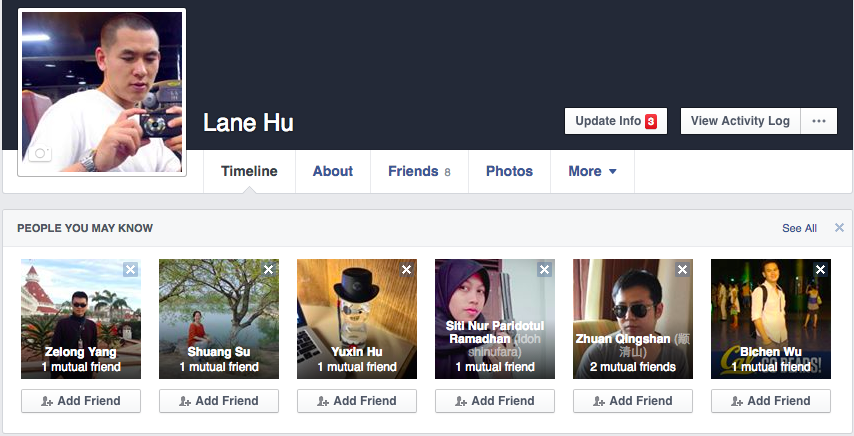
\includegraphics[scale=0.45]{figures/recmd_facebook}}
	      \figcaption{Facebook个性化推荐用户界面}
	      \label{pic:recmd_facebook}
	    \end{figure}
		作为全球社交网站中的翘楚,Facebook在很早的时候就预言到了大数据+推荐系统的无限前景。Facebook自己的推荐系统就是需要利用分布式计算框架快速的帮助用户找到他们可能感兴趣的人、文章、分析、用户组等。Facebook是个伟大的公司,一直为开源软件贡献着一份力量,最近在其官网就公布了facebook自己的推荐系统原理、性能及使用情况\citep{recmd-facebook}。Facebook的推荐系统需要面对的数据量应该是所有互联网公司中的数一数二,约包含了1000亿级别的评分数、10亿级别的用户数以及百万级别的虚拟商品,如何在如此庞大的数据规模下,仍然保持良好性能已经成为世界级的难题,而facebook解决了。即使是采用现在流行的分布式计算框架,Facebook仍然不可能穷举每一对用户-物品的评分。团队需要寻找效率更高、耗时更少的算法来获得每个用户topN的推荐物品,然后再利用推荐系统计算用户对其的评分,这与我们之前解释的恰好相反。解决方案是利用ball tree数据结构存储商品的权重向量。all tree可以贡献搜索过程10-100倍的加速率,使得推荐结果能够在合理时间内完成,代价就是增加了空间使用量,典型的以时间换空间策略。最后,通过分析Facebook给出了一些实验的结果,表明,Facebook的系统比传统系统要快10倍左右。因此可以轻松愉快的处理1000亿级别的评分数据。目前,该方法已经用到Facebook的多个app应用中,包括用户、用户组的推荐。进一步的,为了能够减小系统负担,Facebook只是把稀疏度超过100的用户考虑为候选推荐集合。在初始迭代中,Facebook推荐系统直接把用户历史上喜欢过的主页、群组以及不喜欢的群组都作为输入。最重要的是Facebook还利用ALS算法,从用户获得间接的反馈,这样算是完成推荐-反馈-优化-推荐的一个完美闭环。未来Facebook会继续优化推荐系统,持续改进部分关键模块,包括社交图、用户跳转路径、自动化参数调整以及较好的机器负载均衡策略等。Facebook推荐主页如\autoref{pic:recmd_facebook}。
		
		Facebook的用户画像进展也十分可观,几乎是与推荐系统同步发展。2011年12月,Facebook发布了里程碑式的大数据产品——Timeline,通过开发API接口,允许用户自行编辑个人的时间轴:在什么时间、什么地点做了什么,遇到了谁,可以说在这条时间线记录这个人的全部生活故事。Timeline通过帮用户回忆自己的点点滴滴的同时,完成了用户数据捕获、存储,而一旦拥有了这些历史数据,Facebook就可以做进一步的数据分析、挖掘,这时的Facebook就如同和你从小长大的小伙伴,一个懂你的陌生人。可以说用户留下的数据越多,Facebook就越了解这个人,投放的广告就会更加精准,最终facebook利用庞大的用户数据生态赚足了钱。

		豆瓣网是国内互联网行业中的小清新,美誉度很高,这是一家致力于帮助用户发现美好事物为己任的公司\citep{recmd-douban}。不用费力设置播放列表,也不用费心思考要听啥,打豆瓣电台的推荐栏目,就能获得意想不到的快乐。如初恋般的音乐体验,让用户和音乐不期而遇,豆瓣电台坚持找到符合用户口味音乐。通过高度匹配的推荐结果,豆瓣电台为音乐爱好者提供了这样一种崭新的音乐盛宴,音乐本来就是件轻松的事,豆瓣电台回归了音乐最初定位。豆瓣电台的推荐算法综合用户的各种音乐行为\citep{recmd-doubanFM}。在豆瓣音乐中,通过量化音乐标签,谁喜欢哪些歌手,在听哪些,想听哪些,乐评,豆列等指标,会有相关的权重算法算出一个数值,最开始的时候只是一个最简单的计算公式,在经过多次产品迭代和用户反馈后,得出更靠谱的权重值累加算。其中权重最多的应该是电台本身的红心、踩、跳过、这些显性行为数据。豆瓣电台糅合了包括数据清洗、分析、挖掘、整合、用户画像建模、编辑与运营、后台架构等等大量的因素,如此庞大的架构中,即便是推荐算法也只是现实的一部分。豆瓣电台推荐页如\autoref{pic:recmd_doubanFM}。

		豆瓣电台的用户画像结构大致有俩快:享受时间和购买时间,用户画像的目标用户群体是在线观众,通过用户购买时间差区别并得出分类标签。如通过分析得出此类用户大多数是周末购买音乐工作日静下心慢慢享受。用户年龄、职业和地址,这是根据用户的经纬度和注册信息来对用户进行分类的用户画像建模。用户的经纬度分为一线城市,如北京、上、二线城市,如武汉、深圳、厦门、其他三类,如合肥、呼和浩特。年龄分为小于25岁、26到35岁、36到45岁和46岁以上四类。据统计结果表明:按人群经纬度分布,大致与橄榄球相似,二线城市的人群占中间的大部分,其他城市人数飞速增长;按用户年龄分布,九十后用户占主体地位。同时对情侣关系的用户推荐喜欢度接近的音乐。按活跃程度分布主要分为3档:100次以下;100-300次;300次以上。也可以同时考虑多个维度,包括活跃度、经纬度、年龄段,进行用户画像建模。
		\begin{figure}
	    \centering
	      \framebox{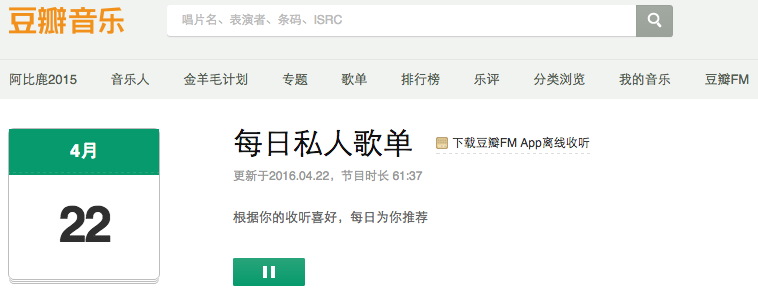
\includegraphics[scale=0.5]{figures/recmd_doubanFM}}
	      \figcaption{豆瓣电台个性化推荐用户界面}
	      \label{pic:recmd_doubanFM}
	    \end{figure}

		\subsection{推荐系统的主要方法}
		推荐系统主要有俩种思路:评分预测和Top-N预测,核心的目标都是找到最适合用户的候选集合s,从候选集合里挑选目标集合是一个非常复杂的非线性优化问题,通常采用的方案是用局部最优近似非线性最优,通过定义一个的损失函数,选取Top-N	\citep{recmd-Next}。
		\begin{enumerate}[(1)]
		\item 协同过滤的推荐

		推荐系统的算法基于统计学、概率论、线性代数、微积分技术,找出用户最有可能喜欢的商品,应该是现代互联网电商的明星应用。目前用的比较广泛的推荐算法还属协同过滤推荐算法,其基本思想是根据与他兴趣相近的用户的选择,得出推荐商品候选集,取topN推荐给目标用户,用维度为m×n的矩阵表示所有用户对所有物品的兴趣值,这个值应该是根据用户历史行为数据得出,值越高表示这个用户越喜欢,利用特殊值0表示没有接触过。图中行向量表示某个用户对所有商品的喜爱程度,列向量表示某个商品对所有用户的吸引程度,因此单个元素$U_{ij}$表示用户i对物品j的喜欢程度。协同过滤分为两个阶段:预测阶段和推荐阶段。预测阶段是基于所有原始集商品,预测这个用户有没有可能对其感兴趣,量化为一个数值,只要值不为零即可归为候选集中;推荐是根据预测结果,先去重后去除消费过的商品,然后根据某种算法去TopN推荐给用户。按照用户-商品数值的得出类型,协同过滤算法分为基于内容的和基于模型俩大类\citep{Wikipedia}。

		协同过滤算法的基本思路是基于一个假设:如果某类用户群对相同商品的打分比较类似,则表明他们的品味从某种程度上类似,由此可以推出在其它类项目的打分也应该类似才对。协同过滤推荐系统先定义好距离计算公式,然后搜索与目标用户相似的其他潜在类似用户,并根据类似用户的打分来量化潜在用户对指定商品的评分,最后选择评分最高的商品列表推荐给用户,同时可以给出令人信服的推荐理由:如某某人也购买过、评价过该商品。这种算法的优点很多:计算简单、精确度较高,能够自圆其说,因此被广泛采用。总之,基于User的协同过滤推荐算法的核心,就是先通过距离计算公式得出类似邻居,然后将最近邻的好评过的商品推荐给目标用户,很简单。

		例如,在\autoref{tab:User-based}所示的用户一商品评分矩阵中,行向量代表用户,列向量代表电影。表中的数值代表用户对电影的评价量化后的值。现在需要预测用户Hanmeimei对电影《教父》的评分(用户maggie对电影《X-Files 要你相信》的评分是缺失的数据)。
		由\autoref{tab:User-based}不难发现,Lane和Pony对电影的评分非常接近,Lane对《暮色3:月食》、《唐山大地震》、《X-Files 要你相信》的评分分别为3、4、4,Hanmeimei的评分分别为3、5、4,他们之间的相似度最高,因此Lane是Hanmeimei的最接近的邻居,Lane对《教父》的评分结果对预测值的影响占据最大比例。相比之下,用户Jackson和maggie不是Hanmeimei的最近邻居,因为他们对电影的评分存在很大差距,所以Jackson和maggie对《教父》的评分对预测值的影响相对小一些。
		\begin{table}[htp]
		\centering
		\tabcaption{用户-物品表}
		\label{tab:User-based}
		\begin{tabular}{ |c|p{2cm}|p{2cm}|p{2cm}|p{2cm}| } \hline
		 & 暮色3:月食 & 唐山大地震 & X-Files 要你相信 & 教父 \\ \hline
		Jackson & 4 & 4 & 5 & 4 \\ \hline
		Marry & 3 & 4 & 4 & 2 \\ \hline
		maggie & 2 & 3 &  & 3 \\ \hline
		Hanmeimei & 3 & 5 & 4 &  \\ \hline
		\end{tabular}
		\end{table}
		\end{enumerate}
		尽管有这么多的优点,协同过滤算法也存在两大问题:1、数据稀疏性。一个大型的电子商务平台一般有百万级别的物品,用户可能接触到的商品占所有商品的百分之一不到,因此用户之间购买过的物品重叠性非常小,以至于没办法做推荐,一个办法是利用算法添补部分值\citep{recmd-slopone}。2、扩展性较差,因为一般来讲,电子商务平台中的商品变动很小,用户流入流出、日益增加、变动很大,基于用户的协同过滤算法需要不停的跟新迭代保证跟上用户变动的步伐。遇到这种情况,可以考虑基于商品的协同过滤算法,其基本思想类似于基于用户的协同过滤算法,只是相似性计算对象是商品,而商品一般变动很小可以忽略不计。如果我们知道物品a和b相似,而一般喜欢a的用户也喜欢b,如果用户A喜欢a,那么我们有很大把握得知A也应该喜欢b,推荐了准没错。而物品之间的相似性比较固定,因此可以一次性计算出物品的相似度,将结果存储到redis中,推荐时查询redis即可。

		\subsection{推荐系统评测的测量指标}
		推荐系统存在三个参与方:用户、物品提供者和平台。好的推荐系统总体来说是一个能令三方共赢的系统。那么如何评价推荐系统功效呢? 从用户角度,推荐系统必须满足用户的需求,推荐的应该是那些令用户感兴趣的、之前又没有遇到过的商品,即推荐精度。推荐系统还应该有预测用户行为的功能,通过历史展望未来,帮助用户发现那些他们原本没机会发现的小众商品,即长尾效应。最后推荐系统也应该能引导用户兴趣,推荐一些商品,虽然与用户兴趣无关,但是用户看见可能会产生兴趣的商品,即惊喜度。从平台角度,推荐系统能够让平台的营收上一个台阶。
			\begin{enumerate}[(1)]
			\item 用户满意度

			用户满意度是最难量化的指标,也是最关键的指标。推荐系统的本意就是让用户满意。量化用户满意度可以采用用户问卷调查,还有一种更直接的方式,就是在推荐结果的侧栏设置俩个按钮,方便用户在线实时反馈意见,据笔者所知豆瓣的推荐物品旁边都有这类按钮,而亚马逊另辟蹊径,利用一些关键性指标衡量用户对推荐系统的满意度,一般用点击率,用户停留时间,转化率等指标来度量。
			\item 预测准确度

			如果是评分机制,则一般通过计算预测结果集合与用户实际消费集合直接的重合度,得出推荐系统的准确度。如果是Top-N推荐,则涉及到关键指标:召回率和准确率。准确率指在所有的推荐结果中有多少个是对的,其所占的比重,以推荐结果集合个数当除数。召回率则是指用户实际消费商品集合中,有多少物品出现在推荐结果中,已用户实际消费商品集合个数当除数。
			\item 覆盖率

			就是指推荐系统有没有照顾小众商品,而不是一个劲的推荐热门商品。方法就是统计推荐结果的类型个数,比上所有商品类型个数,得到的商越大代表覆盖率越好,其他方法就涉及到信息学中的熵和基尼系数。
			\item 多样性

			针对某一个用户,推荐结果中要变化多端,不能一根筋的推荐一种类型。比如电影,如果用户即格斗类的电影,同时又喜欢爱装小清新,那么推荐列表中就应该是两个类型的集合,除此之外,适当添补一些小众电影,三者比例按用户的爱好来推荐,比如用户爱格斗片多一点,文艺片也喜欢,历史片只是偶尔,那么推荐结果中最好也跟这个比例大差不差。
			\item 新颖性

			如果系统推荐的物品其实是用户知晓的,那么这就是一次失败的推荐,完全失去了推荐的意义。一般来讲,用户都是期望推荐一些自己暂时还不知道的商品或者没看过没买过的商品。方法之一是过滤掉用户已经看到过、购买过、点击过的物品,除此之外,物品的平均流行度与其新颖度成反比,越冷门的物品越会给用户新颖的感觉。比如用户是周星驰的粉丝,那么推荐《临岐》就是一个很棒的选择,因为很少人知道这是周星驰出演的。
			\item 信任度

			如果一个用户信任推荐系统,那么他不仅会频繁的选择查看推荐结果,还有适时的与推荐系统互动,包括反馈、评价、提建议等。如果用户信任推荐系统,从而获得更好的个性化推荐,这是一个良性循环。
			\item 实时性

			有时候一个推荐系统的实时性的重要性大过天\bibitem{temporal-cf},试想一下,如果一个用要买睡袋,但不知道哪款睡袋好,推荐系统如果这是恰当好处的推荐结果,那么对于用户是很有意义的一件事情。反之,等用户买都买了,推荐系统在作出推荐,只会让用户难堪。
			\end{enumerate}

	\section{本章小结}
	本章简单概述了用户画像的研究现状,讨论了相关的建模过程。然后介绍了推荐系统的主要任务和问题,并从商业应用和学术研究两个角度介绍了推荐系统研究的现状,最后讨论了推荐系统的主要评测指标。